%%\documentclass[tikz, margin=3mm]{standalone}
\documentclass[convert={density=300,size=700x400,outext=.png}]{standalone}
\usepackage{tikz}
\usetikzlibrary{
  shapes,
  calc,
  arrows,
  arrows.meta,
  through,
  intersections,
  positioning,
  decorations,
  trees,
  decorations.pathreplacing,
  decorations.markings}

\begin{document}
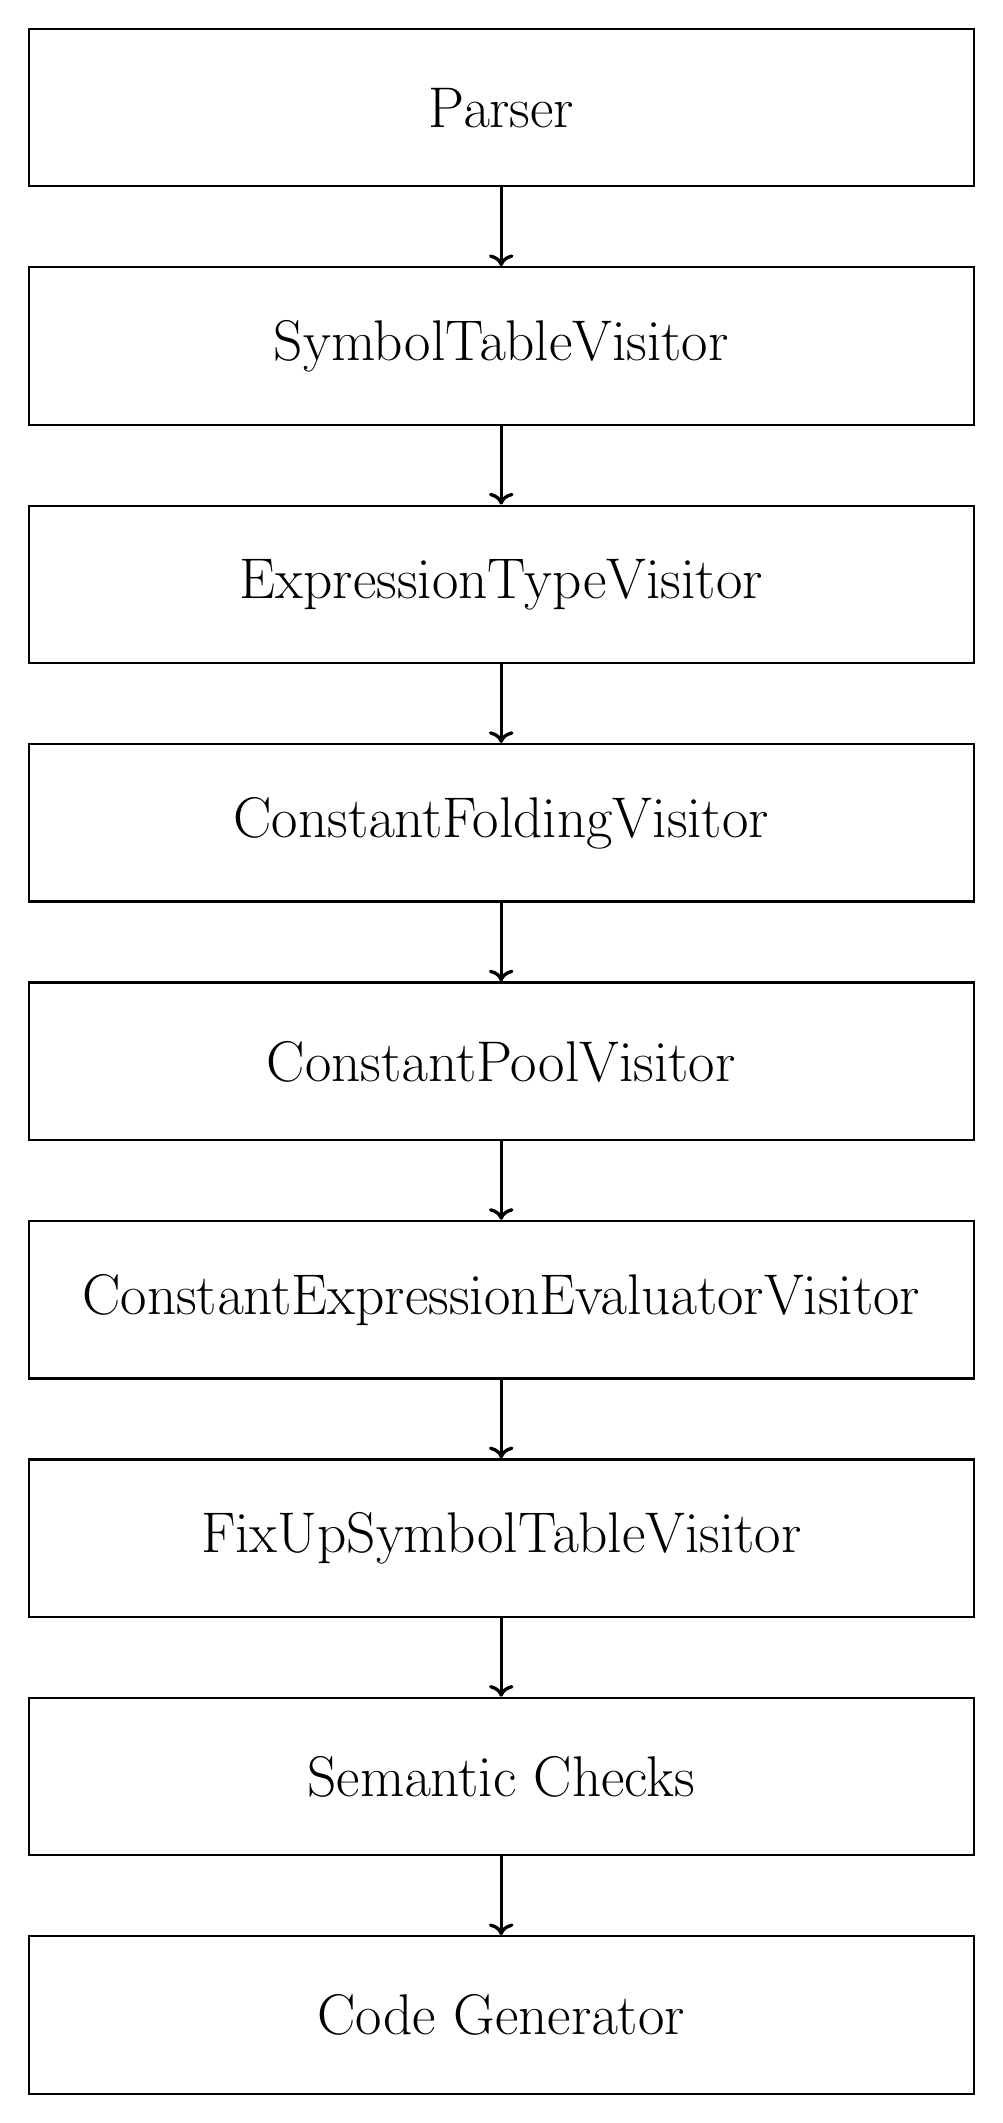
\begin{tikzpicture}[scale=1.0]
  \tikzset{mark coordinate/.style={inner sep=0pt,
                                   outer sep=0pt,
                                   minimum size=3pt,
                                   fill=#1,
                                   circle}
                                   }

%%%%%%%%%%%%%%%%%%%%%%%%%%%%%%%%%%%%%%%%%%%%%%%%%%%%%%%%%%%%%%%%%%%%%%%%%%%%%%

%%\draw [step=0.5,thin,gray!25] (-10cm,-10cm) grid (40cm,20cm);

%%%%%%%%%%%%%%%%%%%%%%%%%%%%%%%%%%%%%%%%%%%%%%%%%%%%%%%%%%%%%%%%%%%%%%%%%%%%%%

\node[draw,rectangle,color=black,thick,minimum width=12cm,minimum height=2cm, align=center, font=\huge] (P) {Parser};

\node[draw,rectangle,color=black,thick,minimum width=12cm,minimum height=2cm,below=of P, align=center, font=\huge] (STV) {SymbolTableVisitor};

\node[draw,rectangle,color=black,thick,minimum width=12cm,minimum height=2cm,below=of STV,font=\huge] (ETV) {ExpressionTypeVisitor};

\node[draw,rectangle,color=black,thick,minimum width=12cm,minimum height=2cm,below=of ETV,font=\huge] (CFV) {ConstantFoldingVisitor};

\node[draw,rectangle,color=black,thick,minimum width=12cm,minimum height=2cm,below=of CFV,font=\huge] (CPV) {ConstantPoolVisitor};

\node[draw,rectangle,color=black,thick,minimum width=12cm,minimum height=2cm,below=of CPV,font=\huge] (CEEV) {ConstantExpressionEvaluatorVisitor};
  
\node[draw,rectangle,color=black,thick,minimum width=12cm,minimum height=2cm,below=of CEEV,font=\huge] (FUSTV) {FixUpSymbolTableVisitor};

\node[draw,rectangle,color=black,thick,minimum width=12cm,minimum height=2cm,below=of FUSTV,font=\huge] (SC) {Semantic Checks};

\node[draw,rectangle,color=black,thick,minimum width=12cm,minimum height=2cm,below=of SC,font=\huge] (CG) {Code Generator};

%%%%%%%%%%%%%%%%%%%%%%%%%%%%%%%%%%%%%%%%%%%%%%%%%%%%%%%%%%%%%%%%%%%%%%%%%%%%%%
\draw[->, very thick]  (P) -- (STV);
\draw[->, very thick]  (STV) -- (ETV);
\draw[->, very thick]  (ETV) -- (CFV);
\draw[->, very thick]  (CFV) -- (CPV);
\draw[->, very thick]  (CPV) -- (CEEV);
\draw[->, very thick]  (CEEV) -- (FUSTV);
\draw[->, very thick]  (FUSTV) -- (SC);
\draw[->, very thick]  (SC) -- (CG);

%%%%%%%%%%%%%%%%%%%%%%%%%%%%%%%%%%%%%%%%%%%%%%%%%%%%%%%%%%%%%%%%%%%%%%%%%%%%%%

\end{tikzpicture}
\end{document}
